\documentclass{article}
\usepackage{tikz}




\begin{document}

\pagestyle{empty}
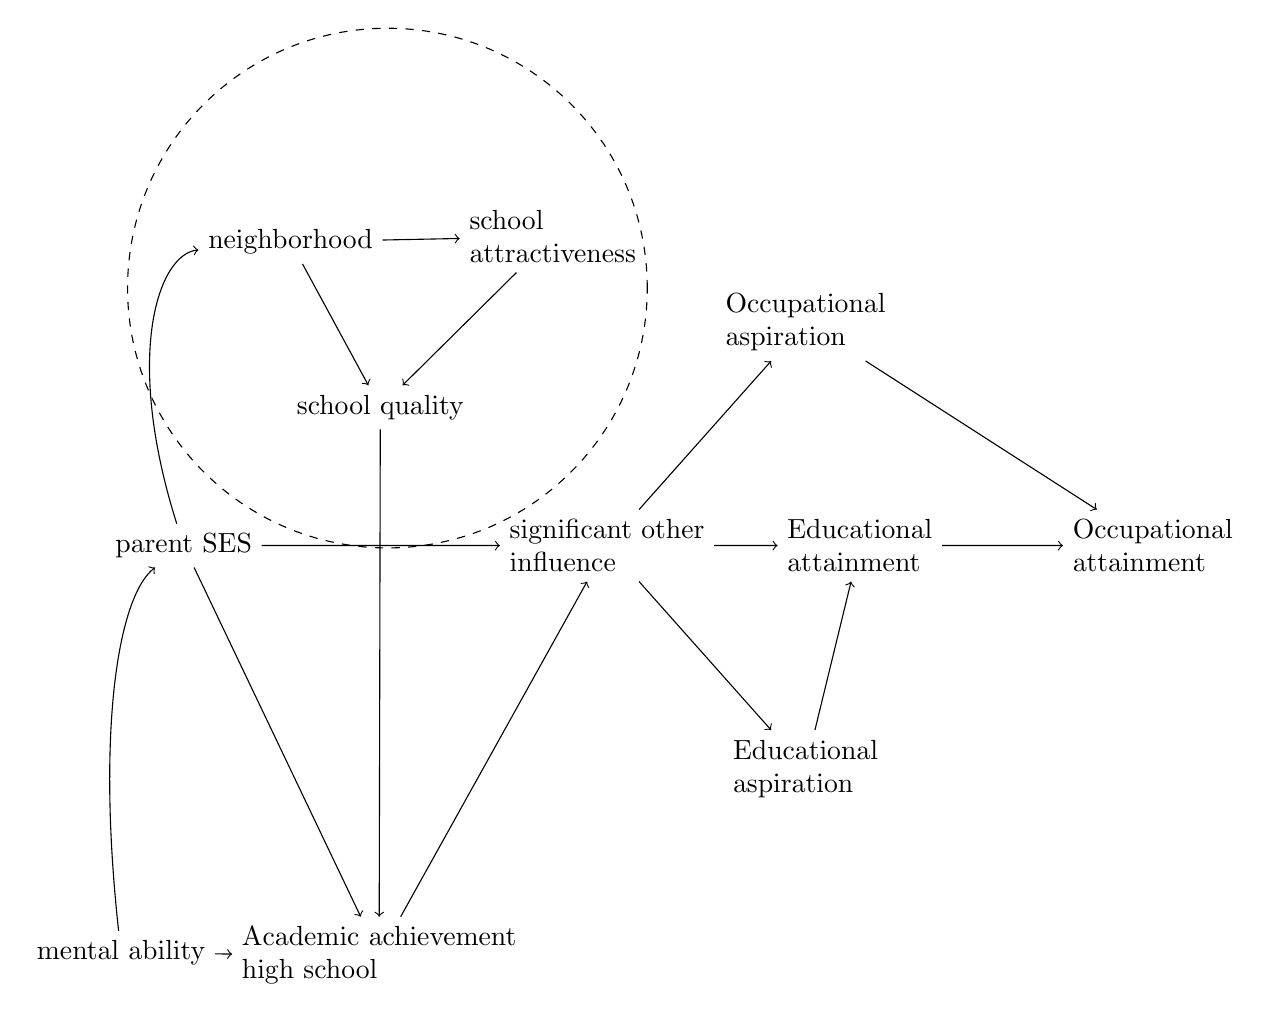
\begin{tikzpicture}[scale=15]
\node (v0) at (0.0875,-0.308) {parent SES};
\node (v1) at (0.178,-0.0509) {neighborhood};
\node (v2) at (0.254,-0.191) {school quality};
\node[align=left] (v3) at (0.400,-0.0464) {school\\attractiveness};
\node[align=left] (v4) at (0.660,-0.308) {Educational\\attainment};
\node[align=left] (v5) at (0.908,-0.308) {Occupational\\attainment};
\node (v6) at (0.0345,-0.653) {mental ability};
\node[align=left] (v7) at (0.253,-0.655) {Academic achievement\\high school};
\node[align=left] (v8) at (0.446,-0.308) {significant other\\influence};
\node[align=left] (v9) at (0.614,-0.497) {Educational\\aspiration};
\node[align=left] (v10) at (0.614,-0.119) {Occupational\\aspiration};
\draw[fill=none, dashed](0.26,-.09) circle (.22) node [black,yshift=-.1cm] {};
\draw [->] (v3) edge (v2);
\draw [->] (v1) edge (v3);
\draw [->] (v1) edge (v2);
\draw [->] (v4) edge (v5);
\draw [->,<-] (v0) .. controls (0.0315,-0.351) and (0.0139,-0.466) .. (v6);
\draw [->] (v6) edge (v7);
\draw [->] (v0) edge (v7);
\draw [->] (v7) edge (v8);
\draw [->] (v0) edge (v8);
\draw [->] (v2) edge (v7);
\draw [->] (v8) edge (v9);
\draw [->] (v8) edge (v10);
\draw [->] (v10) edge (v5);
\draw [->] (v9) edge (v4);
\draw [->] (v8) edge (v4);
\draw [->,<-] (v1) .. controls (0.0663,-0.0607) and (0.0363,-0.146) .. (v0);
\end{tikzpicture}


\end{document}